\section{Результаты численных экспериментов}
\label{section:results}

\subsection{Разработка математической модели}
\label{results:calibration}

%#В данном подразделе приведены исходные данные, оценённые параметры распределений маргиналов и копул, а также приведены результаты goodness-of-fit тестов. В последней главе приведены результаты оптимизации портфеля и сравнение риск метрик оптимального и равновесного портфелей.

\subsubsection{Исходные данные}

В данной работе используется портфель из следующих активов: фьючерсы на акции (1) ГМК <<Норильский Никель>> (GMKR), (2) <<Газпром>> (GAZR) и (3) <<Сбербанк>> (SBRF) и (4) индекс РТС (RTS). 
В качестве исходных данных используются ежедневные цены закрытия вышеперечисленных контрактов с 16 декабря 2015 по 16 декабря 2017 (504 наблюдения). %# во ввдении указана другая длина
Особенность данных временных рядов заключается в том, что в качестве соответствующих контрактов используются <<склеенные>>   фьючерсы \cite{Masteika2012}.
%Таким образом, мы можем иметь дело с длительными наблюдениями. 

В первую очередь, полученные котировки активов были преобразованы в логарифмические доходности через уравнение~(\ref{log-returns}).
На рис.~\ref{ris:hist} изображены гистограммы полученных временных рядов, а в таблице~\ref{tab:assets} указаны их основные характеристики: средняя дневная доходность и стандартное отклонение. Согласно методологии (раздел~\ref{methodology:preparing}), в данной работе мы использовали коэффициент нелинейной ранговой корреляции $\tau$ Кендалла~(\ref{kendall}).

\begin{table}[htb]
    \centering
    \caption{Описательные  характеристики логарифмических доходностей}
    \label{tab:assets}
    \begin{adjustbox}{max width=\textwidth}
    \begin{tabular}{l|cc|rrrr|rrrr}
        \toprule
        \multirow{2}{*}{Активы} & \multicolumn{2}{c|}{Моменты} & \multicolumn{4}{c|}{$\rho$ Спирмена} & \multicolumn{4}{c}{$\tau$ Кендалла} \\
        & $\mu$ & $\sigma$ & \multicolumn{1}{c}{RTS} & \multicolumn{1}{c}{SBRF} & \multicolumn{1}{c}{GAZR} & \multicolumn{1}{c|}{GMKR} & \multicolumn{1}{c}{RTS} & \multicolumn{1}{c}{SBRF} & \multicolumn{1}{c}{GAZR} & \multicolumn{1}{c}{GMKR} \\ 
        \midrule
RTS  &  0.00075 & 0.016 &     1 & 0.702 & 0.621 & 0.323 &     1 & 0.515 & 0.444 & 0.218 \\
SBRF &  0.00154 & 0.016 & 0.702 &     1 & 0.519 & 0.308 & 0.515 &     1 & 0.364 & 0.208 \\
GAZR & -0.00001 & 0.013 & 0.621 & 0.519 &     1 & 0.375 & 0.444 & 0.364 &     1 & 0.256 \\
GMKR &  0.00033 & 0.015 & 0.323 & 0.308 & 0.375 &     1 & 0.218 & 0.208 & 0.256 &     1 \\    
        \bottomrule
    \end{tabular}
    \end{adjustbox}
\end{table}

\imgh[p]{Histogram.pdf}{width=\textwidth}{Гистограммы лог-доходностей активов, включенных в портфель}{hist}

\subsubsection{Результаты оценки параметров распределений}
\label{calibration:marginals}

\begin{table}[!b]
\centering
\caption{Оценка параметров маргинальных распределений}
\label{tab:marginals}
\setlength{\tabcolsep}{5pt}
\begin{tabular}{lcrrrr}
\toprule \multicolumn{2}{c}{Параметры} & \multicolumn{1}{c}{RTS} &
\multicolumn{1}{c}{SBRF} & \multicolumn{1}{c}{GAZR} &
\multicolumn{1}{c}{GMKR} \\ \midrule[1pt]
\multirow{4}{*}{\begin{tabular}{l}
    Гиперболическое \\
    распределение 
\end{tabular}}
    &    $\pi$ &    0.00336 &    0.06100 &    0.06751 &    0.03301 \\
    &  $\zeta$ &    0.68417 &    0.80977 &    0.73310 &    3.31449 \\
    & $\delta$ &    0.00694	&    0.00823 &    0.00609 &    0.02232 \\
    &    $\mu$ &    0.00067 & $-$0.00003 & $-$0.00139 & $-$0.00076 \\ \midrule
\multirow{4}{*}{\begin{tabular}{l}
    Устойчивое \\
    распределение
\end{tabular}}
    & $\alpha$ &    1.53561 &    1.56414 &    1.86326 &    1.92994 \\
    &  $\beta$ &    0.21114 &    0.22262 &    0.85066 &    0.66465 \\
    & $\gamma$ &    0.00884 &    0.00926 &    0.00770 &    0.00999 \\
    & $\delta$ &    0.00020 &    0.00063 & $-$0.00099 & $-$0.00016 \\ \midrule
\multirow{4}{*}{\begin{tabular}{l}
    Распределение \\
    Мейкснера 
\end{tabular}}
    & $\alpha$ &    0.03306 &    0.03064 &    0.02642 &    0.00428 \\
    &  $\beta$ &    0.30800 &    0.45599 &    0.22236 &    0.87412 \\
    & $\delta$ &    0.44168 &    0.51881 &    0.47397 &   18.31193 \\
    &    $\mu$ & $-$0.00099 & $-$0.00173 & $-$0.00143 & $-$0.03615 \\ \bottomrule
\end{tabular}
\end{table}

Параметры маргинальных распределений оцениваются согласно методологии, описанной в разделе~\ref{methodology:marginals}. Полученные результаты приведены в таблице~\ref{tab:marginals}. 
Результаты тестов для оценки качества полученных результатов -- Колмогорова\,--\,Смирнова, Андерсона\,--\,Дарлинга и Крамера\,--\,фон~Мизеса, -- приведены в таблице~\ref{tab:margintest}.

Для выбора одного распределения будем использовать значения $p$-value, полученные в результате теста Крамера\,--\,фон~Мизеса, который является самым мощным статистическим критерием из рассматриваемых в данной работе. По его результатам мы выбрали распределение Мейкснера в качестве маргинального, которое будем использовать в дальнейших расчетах.
На рис.~\ref{ris:bestmargins} приведены графические результаты оценивания параметров распределений. Слева на рисунке изображены гистограммы лог-доходностей и наложенные на них графики плотности выбранного маргинального распределения Мейкснера. Справа показаны квантиль-квантильные графики для наблюдаемых и модельных данных, полученных с использованием выбранного распределения Мейкснера. Вертикальные пунктирные линии соответсвуют квантилям уровня $0.05$ и $0.95$.

\begin{table}[!t]
\centering
\caption{Значения $p$-value статистических тестов для распределений-кандидатов}
\label{tab:margintest}
\setlength{\tabcolsep}{4pt}
\begin{tabular}{llcccc} \toprule
\multicolumn{1}{c}{Тест} & \multicolumn{1}{c}{Распределение} & RTS & SBRF & GAZR & GMKR \bigstrut \\ \midrule[1pt]
\multirow{3}{*}{\begin{tabular}{l}
    Колмогорова\,--\, \\
    Смирнова
\end{tabular}}
    & Гиперболическое & 0.91 & 0.88 & 1.00 & 0.79 \\
    & Устойчивое      & 0.89 & 0.94 & 0.87 & 0.94 \\
    & Мейкснера       & 0.99 & 0.95 & 1.00 & 0.96 \\ \midrule
\multirow{3}{*}{\begin{tabular}{l}
    Андерсона\,--\, \\
    Дарлинга
\end{tabular}}
    & Гиперболическое & 0.88 & 0.94 & 1.00 & 0.93 \\
    & Устойчивое      & 0.73 & 0.87 & 0.47 & 0.97 \\
    & Мейкснера       & 0.87 & 0.92 & 1.00 & 0.90 \\ \midrule
\multirow{3}{*}{\begin{tabular}{l}
    Крамера\,--\, \\
    фон Мизеса
\end{tabular}}
    & Гиперболическое & 0.94 & 0.89 & 1.00 & 0.90 \\
    & Устойчивое      & 0.97 & 0.92 & 0.94 & 0.98 \\
    & Мейкснера       & 0.99\cellcolor{gray!33} & 0.95\cellcolor{gray!33} & 1.00\cellcolor{gray!33} & 0.98\cellcolor{gray!33} \\ \bottomrule
\end{tabular}
\end{table}

\imgh[p]{BestMargins.pdf}{height=0.9\textheight}{Результаты оценки параметров распределений: гистограммы и модельные кривые (слева) и квантиль-квантильные графики (справа)}{bestmargins}

\subsubsection{Результаты оценки параметров копул}

\imgh[thb]{pobs.png}{width=\textwidth}{Парные графики наблюдений (слева) и псевдо-наблюдений
(справа): на главной диагонали -- гистограммы частных
распределений логарифмических доходностей, выше диагонали --
коэффициент ранговой корреляции $\tau$ Кендалла, ниже диагонали --
точечные графики парных совместных распределений}{pobs}


Выше главной диагонали на рис.~\ref{ris:pobs} приведены значения
коэффициента ранговой корреляции $\tau$ Кендалла, ниже главной
диагонали -- точечные графики парных совместных распределений
реальных наблюдений (слева) и полученных псевдо-наблюдений
(справа), на главной диагонали -- гистограммы частных
распределений. Из рис.~\ref{ris:pobs}, видно, что максимальный
коэффициент ранговой корреляции $\tau$ Кендалла наблюдается между
логарифмическими доходностями RTS и SBRF ($\tau=0,51$), эта
величина сохраняется после отображения доходностей в область
определения копулы по правилу~(\ref{pobs}).


Полученные псевдо-наблюдения далее будем использовать для построения оценок параметров копулярных моделей согласно методологии, описанной в разделе~\ref{methodology:copula}.
% Полученные результаты отображены в таблице~\ref{tab:copfit}.
Итогом данного шага для модели Гауссовой копулы является корреляционная матрица $ \Sigma_{Gauss}$, копулы Стьюдента -- корреляционная матрица $ \Sigma_{t}$ и число степеней свободы $v$. Их значения
%
\begin{equation} \label{gausscopfit}
    \Sigma_{Gauss} = \left(
    \begin{array}{cccc}
        1 & & & \\
        0.723 & 1 & & \\
        0.642 & 0.540 & 1 & \\
        0.335 & 0.320 & 0.391 & 1
    \end{array} \right),
\end{equation}

\begin{equation} \label{tcopfit}
    \Sigma_t = \left(
    \begin{array}{cccc}
        1 & & & \\
        0.723 & 1 & & \\
        0.642 & 0.540 & 1 & \\
        0.335 & 0.320 & 0.391 & 1
    \end{array} \right), \ \nu = 4.
\end{equation}
%
Как можно заметить, корреляционные матрицы для обеих копул идентичны. %
Это происходит потому, что оценка первого параметра многомерной копулы определяется только зависимостью между переменными.

Пусть каждому из активов \{RTS, SBRF, GAZR, GMKR\} портфеля соответствует ряд псевдо-наблюдений $u_i$, где $i$ -- порядковый номер актива, $i \in \overline{1,d}$. 
Тогда оценку параметров для вайн копулы можно описать следующей структурой:
%
\begin{enumerate}[label=(\roman*),leftmargin=1cm,labelwidth=1cm]
    \item Дерево 1:\\
    $c_{u_1;u_2}$ -- копула Стьюдента с параметрами $\rho=0.72$, $\nu=7.57$, $\tau=0.51$;\\
    $c_{u_3;u_1}$ -- копула Survival BB1 (повёрнутая на $180^{\circ}$ копула Клейтона-Гумбеля) с параметрами $\theta=0.12$, $\delta=1.68$, $\tau=0.44$;\\
    $c_{u_4;u_3}$ -- копула Survival Gumbel (повёрнутая на $180^{\circ}$ копула Гумбеля) с параметрами $\delta=1.33$, $\tau=0.25$;
    \item Дерево 2:\\
    $c_{u_3,u_2;u_1}$ -- копула Гумбеля с параметрами $\delta=1.1$, $\tau=0.09$;\\
    $c_{u_4,u_1;u_3}$ -- копула Клейтона с параметрами $\delta=0.16$, $\tau=0.07$;
    \item Дерево 3:\\
    $c_{u_4,u_2;u_3,u_1}$ -- копула Франка с параметрами $\delta=0.54$, $\tau=0.06$.
\end{enumerate}
%№ добавить рисунки с указанными деревьями

Эта же структура может быть представлена в виде набора матриц $M$, $F$, $P_1$ и $P_2$, показанных в ур.~(\ref{vinefit}). 
Матрица $M$ определяет структуру дерева, остальные матрицы -- $F$, $P_1$ и $P_2$ -- указывают для каждого узла (парной копулы) набор семейств, первый и второй параметры соответственно. 
Если копула имеет только один параметр, то таковым является $\delta$, если же копула двух-параметрическая, то первым и вторым параметрами являются $\theta$ и $\delta$ соответственно.
В матрице $F$ введены сокращения для обозначения семейств: $St$ -- Стьюдента, $Gu$ -- Гумбеля, $Cl$ -- Клейтона, $Fr$ -- Франка, $SBB1$ -- Survival BB1, $SG$ -- Survival Gumbel.
%
\begin{gather} \label{vinefit}
    M = \left(
        \begin{array}{cccc}
        2 &   &   &   \\
        4 & 1 &   &   \\
        3 & 4 & 3 &   \\
        1 & 3 & 4 & 4 \\
        \end{array} \right), \ \
    F = \left(
        \begin{array}{lll}%{*4{C{5em}}}
        Fr\ &\  &    \\
        Gu\ &\ Cl\ &   \\
        St\ &\ SBB1\ &\ SG\
        \end{array} \right),\\    
    P_1 = \left(
        \begin{array}{ccc}
        0.544 & & \\
        1.098 & 0.158 & \\
        0.722 & 0.124 & 1.327
        \end{array} \right), \ \
    P_2 = \left(
        \begin{array}{ccc}
        0 &  & \\
        0 & 0 & \\
        7.566 & 1.682 & 0
        \end{array} \right). \nonumber
\end{gather}

% Тестирование ----
Результаты статистических тестов полученных моделей приведены в таблице~\ref{tab:coptest}.
Для многомерных Гауссовой и Стьюдента копул был рассчитан функционал Крамера\,--\,фон~Мизеса, а для вайн копулы -- статистика Уайта.
Основываясь на значение $p$-value GoF-тестов оценки параметров, у нас нет основании отвергать нулевую гипотезу о принадлежности копул одному из распределений на 5\% уровне значимости.
Однако по их значениям для R-vine копулы можно заключить, что эта модель является наиболее адекватной из всех по отношению к реальным данным.

\begin{table}[h]
\centering
\caption{Значения статистичеческих критериев для различных копулярных моделей}
\label{tab:coptest}
\setlength{\tabcolsep}{8pt}
\begin{tabular}{lrr}
\toprule
Копула & Статистика & $p$-value \\ \midrule
Гауссова  & $S_n=0.034$ & 0.19 \\
Стьюдента & $S_n=0.391$ & 0.05 \\
R-vine    & $W=15.15$   & 0.95    \\ \bottomrule
\end{tabular}
\end{table}

\subsubsection{Результаты решения задачи поиска оптимального инвестиционного портфеля}
\label{calibration:optim}

В результате решения оптимизационной задачи (\ref{ES})-(\ref{conES}) мы получили портфель, при минимальной доходности портфеля $\bar{\mu}_p=0,05$,  со следующей структурой: $$\textbf{w} = (0.05, 0.114, 0.384, 0.452),$$ здесь каждый элемент вектора -- это доля вложения активов RTS, SBRF, GAZR, GMKR соответственно.
Для того, чтобы убедиться в целесообразности выполнения оптимизации, мы сравнили риск-метрики полученного портфеля со значениями, полученными для равновесного портфеля.
Для данного сравнения можно обойтись обычным историческим методом расчёта VaR и CVaR.
В качестве уровней риск-метрик выберем следующие значения вероятностей $$\pmb{\upalpha} = (90, 95, 99, 99.5, 99.9).$$

\begin{table}[h]
    \caption{Сравнение равновесного и оптимального портфеля для различных вероятностей} \label{tab:eqw-optim}
    \centering
    \setlength{\tabcolsep}{5pt}
    \begin{tabularx}{0.8\textwidth}
    % {c *{3}{|r@{\,/\,}l}} 
    {>{\setlength{\hsize}{\hsize}}Y 
    *{3}{>{\setlength{\hsize}{\hsize}}R
    @{\ /\ }>{\setlength{\hsize}{\hsize}}X}}
    \toprule
\multirow{2}{*}{$\upalpha$, \%} & \multicolumn{6}{c}{$\emph{VaR}_\alpha$ / $\emph{CVaR}_\alpha$, $\times 10^{-2}$} \\ \cmidrule{2-7} 
& \multicolumn{2}{c}{Оптимальный} & \multicolumn{2}{c}{Равновесный} & \multicolumn{2}{c}{Смещение, $\times 10^{-2}$} \\ \midrule
90.0 & $1.31$ & $2.01$ & $1.32$ & $2.14$ & $0.01$ & $0.13$ \\ 
95.0 & $1.69$ & $2.48$ & $1.82$ & $2.74$ & $0.13$ & $0.25$ \\ 
99.0 & $2.59$ & $3.96$ & $2.79$ & $4.36$ & $0.21$ & $0.41$ \\ 
99.5 & $3.63$ & $5.22$ & $4.05$ & $5.50$ & $0.43$ & $0.28$ \\ 
99.9 & $5.62$ & $5.86$ & $6.05$ & $6.29$ & $0.44$ & $0.43$ \\ 
\bottomrule
    \end{tabularx}
\end{table}

В таблице~\ref{tab:eqw-optim} приведены значения риск-метрик для двух портфелей (оптимальный и равновесный) и пяти уровней. 
Четвёртая колонка в таблице показывает разницу между результатами, равную абсолютной разности риск-метрик, полученных для равновесного и оптимального портфелей. 
Из таблицы видно~\ref{tab:eqw-optim}, что при расчёте как VaR, так и CVaR для всех заданных уровней оптимальный портфель показал более консервативную оценку.
Это говорит о целесообразности выполнения оптимизации портфеля.

\subsection{Вычисление риск-метрик с использованием копулярных моделей}
\label{results:risk-measures}

%В данном подразделе приведёны результаты расчётов VaR и CVaR с использованием выбранных моделей копула. Далее проведена бутстрап-процедура с целью получения несмещённой оценки риск метрик. В последней главе получены кривые VaR и CVaR в реальном времени, проведён тест Купича.

\subsubsection{Точечные оценки значений риск-метрик VaR и CVaR}

Для расчета риск-метрик на данном этапе будем использовать массив лог-доходностей с оцененными  для каждой переменной параметрами маргинального распределения Мейснера, весовые коэффициенты найденного CVaR-оптимального портфеля, три копулярных модели с найденными параметрами.
Для заданного в разделе~\ref{calibration:optim} вектора уровней вероятностей $\pmb{\upalpha}$ вычислим значения $\emph{VaR}_\alpha$ и $\emph{CVaR}_\alpha$ согласно алгоритму~\ref{Alg1}.

\begin{table}[bth]
\centering
\caption{Значение  эмпирической $\widehat{VaR}$ и оценённой риск-метрики $VaR^{est}$ c изпользованмием Гауссовой\,/\,Стьюдента\,/\,R-vine копул}
\label{tab:var}
\setlength{\tabcolsep}{5pt}
\begin{adjustbox}{max width=\textwidth}
\begin{tabularx}{\textwidth}{
>{\setlength{\hsize}{\hsize}}Y|
>{\setlength{\hsize}{\hsize}}Y
*{2}{|>{\setlength{\hsize}{0.4\hsize}}R
*{2}{@{\,/\,}>{\setlength{\hsize}{0.4\hsize}}R}}}
\toprule
\multicolumn{1}{c|}{Уровень, \%} & \multicolumn{1}{c|}{$\widehat{\emph{VaR}}$, $\times 10^{-2}$} & \multicolumn{3}{c|}{$\emph{VaR}^{est}$, $\times 10^{-2}$} & \multicolumn{3}{c}{$\Delta$, $\times 10^{-3}$} \bigstrut[t] \\ \midrule
90.0   & $1.31$ & $1.57$ & $1.71$ & $1.51$ & $2.55$ & $3.94$ & $1.94$ \\ 
95.0   & $1.69$ & $2.15$ & $2.37$ & $1.94$ & $4.56$ & $6.81$ & $2.48$ \\ 
99.0   & $2.59$ & $3.28$ & $3.64$ & $3.28$ & $6.95$ & $10.54$ & $6.97$ \\ 
99.5 & $3.63$ & $3.70$ & $4.02$ & $3.94$ & $0.69$ & $3.95$ & $3.13$ \\ 
99.9 & $5.62$ & $5.63$ & $5.83$ & $6.01$ & $0.12$ & $2.18$ & $3.90$ \\ \bottomrule
\end{tabularx}
\end{adjustbox}
\end{table}

\begin{table}[bth]
\centering
\caption{Значение  эмпирической $\widehat{CVaR}$ и оценённой риск-метрики $CVaR^{est}$ c изпользованмием Гауссовой\,/\,Стьюдента\,/\,R-vine копул}
\label{tab:es}
\setlength{\tabcolsep}{5pt}
\begin{adjustbox}{max width=\textwidth}
\begin{tabularx}{\textwidth}{
>{\setlength{\hsize}{\hsize}}Y|
>{\setlength{\hsize}{\hsize}}Y
*{2}{|>{\setlength{\hsize}{0.4\hsize}}R
*{2}{@{\,/\,}>{\setlength{\hsize}{0.4\hsize}}R}}}
\toprule 
\multicolumn{1}{c|}{Уровень, \%} & \multicolumn{1}{c|}{$\widehat{\emph{CVaR}}$, $\times 10^{-2}$} & \multicolumn{3}{c|}{$\emph{CVaR}^{est}$, $\times 10^{-2}$} & \multicolumn{3}{c}{$\Delta$, $\times 10^{-3}$} \bigstrut[t] \\ \midrule
90.0   & $2.01$ & $2.38$ & $2.58$ & $2.32$ & $3.68$ & $5.66$ & $3.12$ \\ 
95.0   & $2.48$ & $2.95$ & $3.17$ & $2.92$ & $4.65$ & $6.89$ & $4.35$ \\ 
99.0   & $3.96$ & $4.25$ & $4.35$ & $4.50$ & $2.98$ & $3.94$ & $5.41$ \\ 
99.5 & $5.22$ & $5.05$ & $4.95$ & $5.43$ & $-1.76$ & $-2.72$ & $2.06$ \\ 
99.9 & $5.86$ & $5.81$ & $6.00$ & $6.01$ & $-0.51$ & $1.38$ & $1.51$ \\ \bottomrule
\end{tabularx}
\end{adjustbox}
\end{table}

\imgh[tbh!]{VaR-ES.pdf}{width=\textwidth}{Точечные оценки риск-метрик VaR (слева) и CVaR (справа) для различых копулярных моделей в сравнении с эмпирическими данными}{smplfied-rm}

В таблицих~\ref{tab:var} и \ref{tab:es} приведены результаты упрощённого расчёта VaR и CVaR соответсвенно.
На рисунке~\ref{ris:smplfied-rm} изображены графики риск-метрик: VaR (слева) и CVaR (справа). 
Из таблиц~\ref{tab:var} и \ref{tab:es} и рисунка~\ref{ris:smplfied-rm} видно, что все три модели остаются консервативными на небольших и средних уровнях вероятности. 
Причём оценки, полученные с помощью Гауссовой и Стьюдента копул, консервативнее по сравнению с более точной моделью R-вайн копулы.
Далее, на уровнях $99.5$ и $99.9\%$ модели Гауссовой и Стьюдента копул начинают вести себя агрессивно (недооценивают риск), в то время как R-вайн остаётся консервативной.
На данном этапе можно сделать выбор в пользу R-вайн копулы, затем копулы Стьюдента и в последнюю очередь Гауссовой как наименее консервативной.
%Однако нам необходимо получить оценку, которую с большей уверенностью можно считать несмещённой.

\subsubsection{Интервальные оценки риск-метрик VaR и CVaR}

Обоснование для использования бутстрап-процедуры описано в разделе~\ref{methodology:bootstrap}.
Для расчётов мы использовали предложенный алгоритм~\ref{Alg2}.
Результаты вычислений для $N=200$ итераций приведены в таблицах~\ref{tab:boot-var} и \ref{tab:boot-es} и на рисунке~\ref{ris:boot-rm}.

Как видно, средние значения для всех трёх моделей очень близки друг к другу.
Вертикальные линии на рисунке~\ref{ris:boot-rm} показывают доверительный интервал от 2.5\% до 97.5\%-ной квантили на каждом уровне, вычисленные по правилу~(\ref{boot-conf-area}).
Этот интервал увеличивается с ростом уровня $\alpha$ для обеих риск-метрик, следовательно, для более точного вычисления меры риска на больших значениях $\alpha$ необходимо использовать большее количество наблюдений.
Величина $\Delta$ показывает смещение средних значений риск-метрик от эмпирических. 
Можно заметить, что все три модели теряют свою консервативность на уровне 99.5 и 99.9\%.
Следовательно, что исследуемая модель работеает для уровней не больше 99\%, что для финансовых моделей вполне достаточно.

\begin{table}[hbt]
\centering
\caption{Характеристики для риск-метрики VaR, полученные с использованием бутстрап-процедуры для  Гауссовой\,/\,Стьюдента\,/\,R-vine копул}
\label{tab:boot-var}
\setlength{\tabcolsep}{5pt}
\begin{adjustbox}{max width=\textwidth}
\begin{tabular}{c*{4}{|r@{\,/\,}r@{\,/\,}r}} \toprule
\multicolumn{1}{c|}{Уровень, \%} & \multicolumn{3}{c|}{$\overline{\emph{VaR}}_\alpha$, $\times 10^{-2}$} & \multicolumn{3}{c|}{$\Delta, \times 10^{-3}$} & \multicolumn{3}{c|}{SD, $\times 10^{-2}$} & \multicolumn{3}{c}{RMSE, $\times 10^{-3}$} \\ \midrule
90.0   & $1.61$ & $1.62$ & $1.61$ & $2.99$ &  $3.03$ &  $2.96$ & $0.80$ & $0.79$ & $0.85$ & $3.10$ & $3.13$ & $3.08$ \\
95.0   & $2.19$ & $2.20$ & $2.18$ & $5.00$ &  $5.06$ &  $4.93$ & $1.18$ & $1.37$ & $1.48$ & $5.14$ & $5.24$ & $5.14$ \\
99.0   & $3.46$ & $3.50$ & $3.46$ & $8.71$ &  $9.11$ &  $8.78$ & $1.79$ & $2.32$ & $2.47$ & $8.89$ & $9.40$ & $9.11$ \\
99.5 & $4.04$ & $4.21$ & $4.09$ & $4.15$ &  $5.82$ &  $4.64$ & $4.22$ & $6.10$ & $5.69$ & $5.91$ & $8.42$ & $7.33$ \\
99.9 & $5.62$ & $5.53$ & $5.49$ & $0.05$ & $-0.86$ & $-1.21$ & $3.81$ & $5.18$ & $5.16$ & $3.81$ & $5.24$ & $5.29$ \\ \bottomrule
\end{tabular}
\end{adjustbox}
\end{table}

\begin{table}[hbt]
\centering
\caption{Характеристики для риск-метрики СVaR, полученные с использованием бутстрап-процедуры для  Гауссовой\,/\,Стьюдента\,/\,R-vine копул}
\label{tab:boot-es}
\setlength{\tabcolsep}{5pt}
\begin{adjustbox}{max width=\textwidth}
\begin{tabular}{c*{4}{|r@{\,/\,}r@{\,/\,}r}} \toprule
\multicolumn{1}{c|}{Уровень, \%} & \multicolumn{3}{c|}{$\overline{\emph{CVaR}}_\alpha$, $\times 10^{-2}$} & \multicolumn{3}{c|}{$\Delta, \times 10^{-3}$} & \multicolumn{3}{c|}{SD, $\times 10^{-2}$} & \multicolumn{3}{c}{RMSE, $\times 10^{-3}$} \\ \midrule
90.0   & $2.46$ & $2.47$ & $2.45$ &  $4.53$ &  $4.62$ &  $4.43$ & $1.08$ & $1.32$ & $1.35$ & $4.66$ & $4.80$ & $4.63$ \\ 
95.0   & $3.06$ & $3.08$ & $3.05$ &  $5.78$ &  $5.92$ &  $5.62$ & $1.49$ & $1.90$ & $1.91$ & $5.97$ & $6.21$ & $5.93$ \\ 
99.0   & $4.36$ & $4.40$ & $4.34$ &  $4.08$ &  $4.46$ &  $3.86$ & $3.05$ & $4.31$ & $4.21$ & $5.09$ & $6.19$ & $5.71$ \\ 
99.5 & $5.00$ & $4.99$ & $4.94$ & $-2.26$ & $-2.31$ & $-2.86$ & $4.05$ & $5.40$ & $5.34$ & $4.63$ & $5.87$ & $6.05$ \\ 
99.9 & $5.76$ & $5.68$ & $5.68$ & $-1.03$ & $-1.79$ & $-1.88$ & $2.45$ & $3.86$ & $3.52$ & $2.65$ & $4.25$ & $3.98$ \\ \bottomrule
\end{tabular}
\end{adjustbox}
\end{table}

\imgh[bth!]{VaR-ES-Bootstrap.pdf}{width=\textwidth}{Интервальные оценки риск-метрик: VaR (слева) и CVaR (справа) в сравнении с эмпирическими данными. Вертикальные линии -- доверительный интервал от 2.5\% до 97.5\%-ной квантили на каждом уровне $\alpha$, $N=200$ итераций}{boot-rm}

\subsubsection{Моделирование кривых VaR и CVaR с использованием копулярных моделей}
\label{riskmeasures:curve}

Выбрав для обучения копулярных моделей первые три месяца, мы построили кривые VaR и CVaR на уровне 95\% и проверили 
их адекватность
с использованием теста Купича.
В качестве <<эталонных>> мы использовали кривые риск-метрик, полученные методом исторического моделирования, описанного уравнениями (\ref{VaR-hist}) и (\ref{ES-hist}).
По результатам на рис.~\ref{ris:VaR-ES-curve} 
% и \ref{ris:ES-curve} %
видно, что все три модели копул являются консвервативными (все модельные кривые лежат ниже кривой P\&L), причём модель R-вайн оценивает риск точнее остальных.

По результатам теста Купича для кривых VaR (таблица~\ref{tab:kupiec}) модель $t$-копула является неадекватной и не может быть использована для оценки риска в реальном времени.
Данные результаты согласуются с результатами GoF-тестов (табл.~\ref{tab:coptest}), в которых было получено крайнее значение $p$-value для $t$-копулы.

\begin{table}[hbt!]
    \centering
    \caption{Значение статистики $LR$ и $p$-value теста Купича для кривых VaR при уровне 95\%}
    \label{tab:kupiec}
    \setlength{\tabcolsep}{10pt}
    \begin{tabular}{lcc} \toprule
        Метод & LR-статистика & $p$-value \\ \midrule
        эмпирический & 0.00 & 0.98 \\
        Гауссова копула & 3.02 & 0.08 \\
        $t$-копула & 10.29 & 0.00 \\
        R-vine & 2.17 & 0.14 \\ \bottomrule
    \end{tabular}
\end{table}

% \imgh[thb!]{VaRcurve.pdf}{width=\textwidth}{График P\&L и кривые VaR}{VaR-curve}
% \imgh[thb!]{EScurve.pdf}{width=\textwidth}{График P\&L и кривые CVaR}{ES-curve}

\begin{figure}[p]
    \centering
    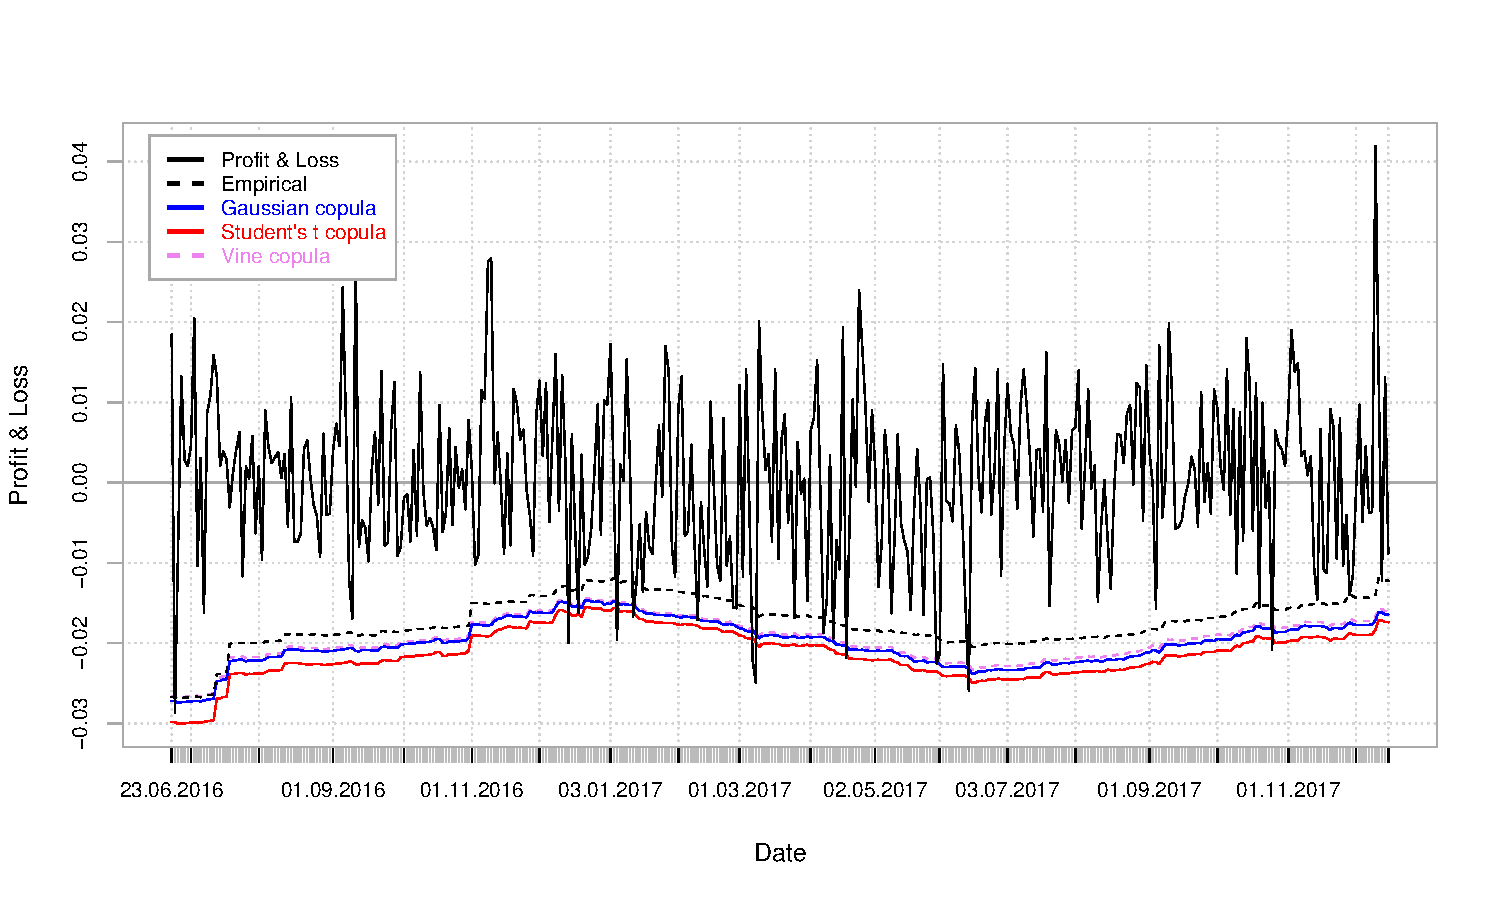
\includegraphics[width=\textwidth]{VaRcurve.pdf}
    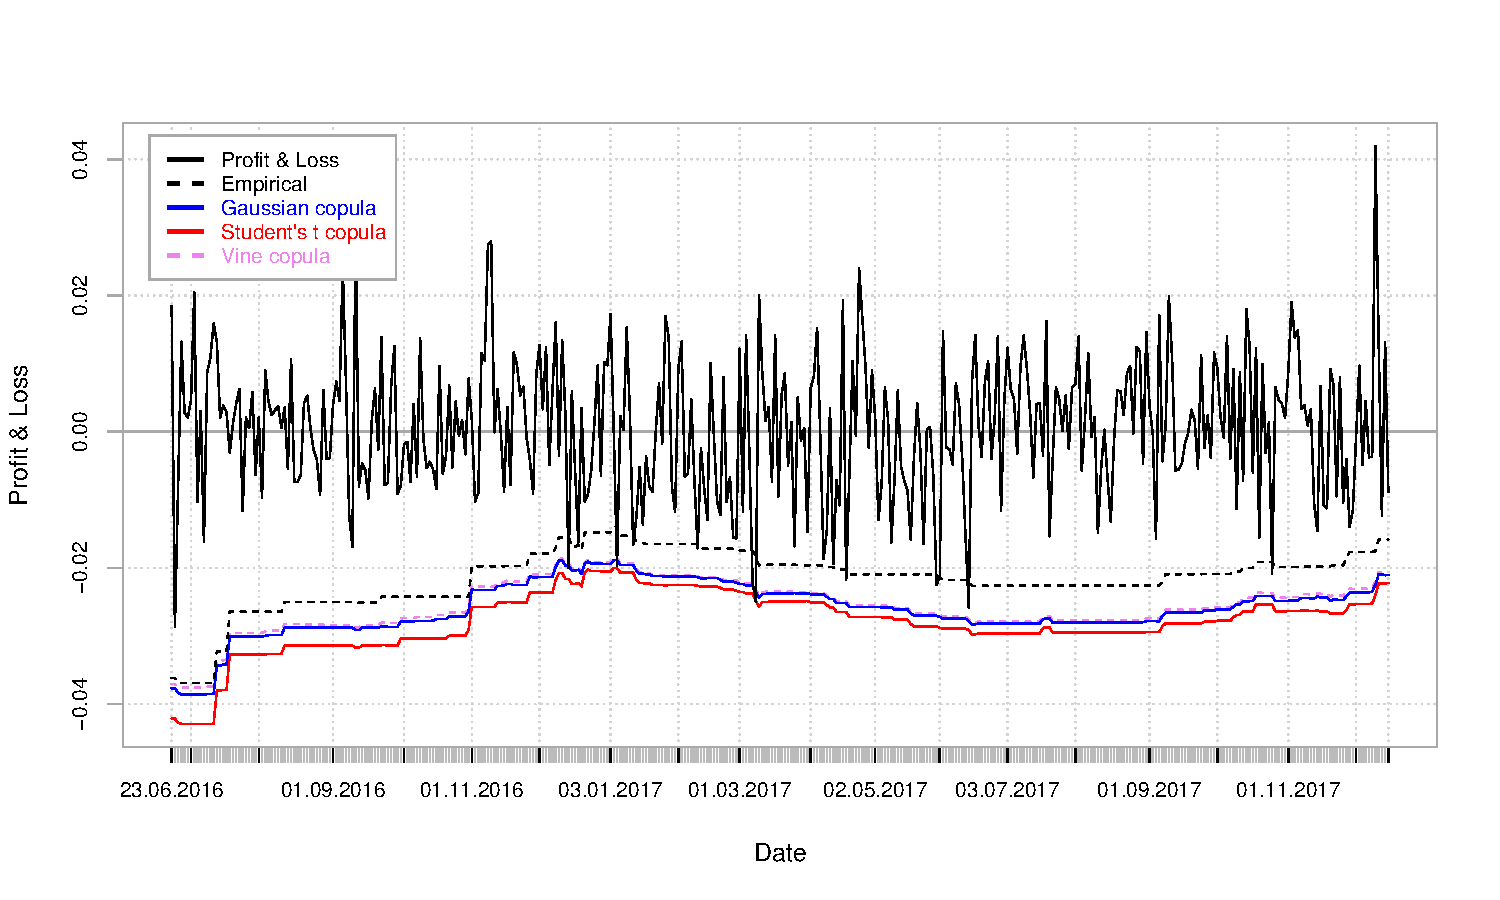
\includegraphics[width=\textwidth]{EScurve.pdf}
    \caption{Смоделированные ряды мер риска VaR (сверху) и CVaR (снизу)
    для различных копулярных моделей в сравнении с эмпирически наблюдаемыми значениями}
    \label{ris:VaR-ES-curve}
\end{figure}
%# уточнить -- эмпирические, P&L. Добавить вертикальную линию, которая будет разделять данные:  для обучения и  модельные